% LaTeX Article Template
\documentclass{article}
\usepackage{amssymb, amsmath, amsfonts, amsthm, latexsym, graphicx, enumitem, tocloft}
\newcommand{\C}{\mathbb {C}}
\newcommand\tab[1][1cm]{\hspace*{#1}}
\newcommand\smalltab[1][0.3cm]{\hspace*{#1}}
\setcounter{section}{-1}
\title{CSCI 362 Final Project: SugarLabs}
\author{Alex Skiff, Blaine Billings, Carson Barber, Chase Myers, Justin Willis}
\date{ }

\renewcommand*\contentsname{Table of Contents}
 
\begin{document}

\begin{titlepage}
    \begin{center}
        \vspace*{1cm}
 
        \Huge
        \textbf{Sugar Labs Automated Testing Framework}
 
        \vspace{0.5cm}
        \LARGE
        CSCI 362 Final Project
 
        \vspace{1.5cm}
 
        \textbf{Alex Skiff, Blaine Billings,}\\
        \textbf{Carson Barber, Chase Myers,}\\
        \textbf{Justin Willis}
 
        \vfill
 
        A framework presented for the automated testing\\
        of the Sugar Labs software project
 
        \vspace{0.8cm}
 
		
\includegraphics[width=0.6\textwidth]{../imgs/ChocolateLeclairs.png}

        \Large
        College of Charleston\\
        CSCI 362: Software Engineering\\
        Dr. Anthony P. Leclerc\\
        30 November 2018
 
    \end{center}
\end{titlepage}
 
\tableofcontents

\newpage

\section{Introduction}
\subsection{Project Description}
Sugar Labs\footnote{https://github.com/sugarlabs} is a free, open-source software that aims to inreases accessibility and ease of use for classroom-setting technology-based learning. Through the project, the developers hope to provide students with an easy to understand and fun learning environment for both the technological sciences and the basics of elementary education. Thier code consists of two main parts - a highly interactive and graphics-based front-end supported by a logical, decision-driven back-end that manages user data, journal logs, learning assignments, and all other relevant materials.

\begin{figure}
\centering

\includegraphics[scale=0.5]{../imgs/Figure4.png}
\end{figure}

While the project's organization follows the software engineering design principle of "separation of powers", dividing up individual tasks among many disjoint pieces of code, the tests associated with each section are neither easily accessible nor comprehensive. This is the problem we aimed to tackle.
\subsection{Testing Framework}
Through our work, we aim to create an automated testing framework that both highly increases the coverage of unit testing, allowing for the verification and near guarantee of fewer program faults, and allows a user of the Sugar Labs software to be able to easily integrate their tests as well as provide additional testing input for existing test classes.

This document is organized as follows. In Section 2, we thoroughly detail how to properly install the Sugar Labs project, accounting for all nececssary software requirements and pre-installation command procedures. Section 3 introduces the testing plan, detailing the specifics of the five principal test cases that serve as an outline for the twenty-five introduced herein. In addition, in this section, we cover various requirements and restraints associated with such an undertaking so as to be prepared for whatever challenges may arise. In Section 4, we provide an architectural description of the automated testing framework, outlining the primary files and folders, as well as discuss in detail the implementation of the five initial test cases as introduced in the previous section. This serves as both a backbone of the testing framework and a guide for any future test cases. In Section 5, we include brief descriptions of all twenty-six implemented test cases, omitting the specifics which can be found in the actual implementation and understood alongisde the models of those characterized in detail in the previous section. In Section 6, we inject faults into the project code so as to demonstrate the veracity of our framework before concluding with a final review.

\section{Deliverable 1: Installation}
\subsection{Clone and Build}
In order to obtain a local instance of the project, we accessed the \textbf{sugar} repository made by the \textbf{SugarLabs} project team on GitHub\footnote{https://github.com/sugarlabs/sugar}. Using the command 
\begin{center}
\textbf{git clone sugarlabs/sugar},
\end{center}
we were, then, able to clone the project to our local machines.

From there, we utilized a document written by the SugarLabs development team included in the root directory, \textbf{README.md}, to guide the process of building the project on the operating system we chose to employ, Ubuntu 16.04. This consisted of running the following commands:
\begin{itemize}
\itemsep-0.5em
\item[] sudo apt-get install sugar-* -y
\item[] aclocal
\item[] sudo apt-get install intltool libglib2.0-dev gtk+-3.0 -y
\item[] ./autogen.sh
\item[] make
\item[] make install
\end{itemize}
\subsection{Existing Tests}
SugarLabs provided multiple testing files for ease of use. After finding the files from the root directory, we searched Python's documentation for \textbf{unittest}, the imported package used for running the test cases. Through the use of this documentation, we were able to get most of the files tested with working output, an example of which is shown in Figure \ref{Figure1}. The commands we used are as follows:
\begin{itemize}
\itemsep-0.5em
\item[] python
\item[] $>>$ import unittest
\item[] $>>$ import FILENAME
\item[] $>>$ x = unittest.TestLoader().loadTestsFromTestCase(FILENAME)
\item[] $>>$ unittest.TextTestRunner(verbosity=2).run(x)
\end{itemize}

Most of the tests passed, with only a few errors thrown. However, despite there being such files nicely laid out, there was neither explanation on how the tests are used nor documentation on what is and is not tested.
\begin{figure}
\centering
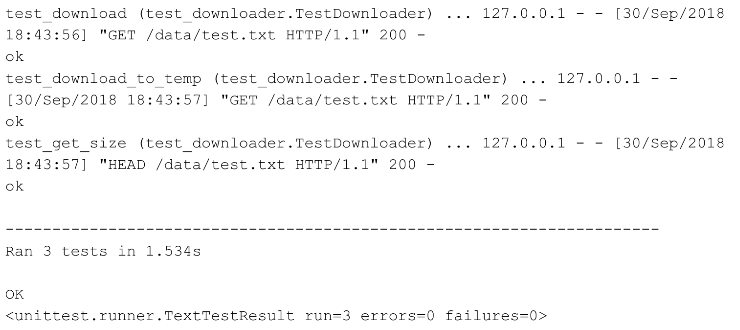
\includegraphics[scale=0.5]{../imgs/Figure1.png}
\caption{A run of an included test file, test\textunderscore downloader.py.}
\label{Figure1}
\end{figure}
\subsection{Team Evaluation}
Overall the project is very organized with some help on building the project provided and only a little lacking information on testing what they have made. The developers were prepared for testing everything they needed to have tested, but only for themselves. It would have been more helpful for others looking in if there was a file that would automate the testing or at least more information on how to set up each individual test. We look forward to creating our own tests and exploring in more detail this project.
\section{Deliverable 2: Introductory Test Plan}
\subsection{Testing Process}
We have divided the process of our test plan for our five introductory test cases into the evaluation of three main subsystems. They are described as follows:
\begin{enumerate}
\itemsep-0.5em
\item \textbf{Profile}: The \textbf{profile} subsystem of SugarLabs includes all files relevant to the creation of a user's profile, including the age, gender, etc. This will be evaluated based on input/ouput matching as well as on exception handling for invalid input.
\item \textbf{Journal}: The \textbf{journal} subsystem of SugarLabs includes all files relevant for the upkeep of a user's journal. Much like with the first subsystem, this will be evaluated based on input/output matching as well as on exception handling for invalid input.
\item \textbf{Activity}: The \textbf{activity} subsystem of SugarLabs includes all files relevant to tracking a user profile's assigned activities, essentially providing running assessment list for the user. This will be evaluated based on correctness of logged information with regards to simulated performed actions.
\end{enumerate}
\subsection{Requirements Traceability}
\label{ReqTrace}
For the aforementioned subsystems, the following files will be evaluated. This information is included for the ease of tracking the testing process and the evaluated files as well as the understanding of what processes in specific are being investigated.
\begin{enumerate}
\itemsep-0.5em
\item \textbf{Profile}: colorpicker.py, agepicker.py, genderpicker.py for color, age, and gender selection, respectively, in the user profile creation process.
\item \textbf{Journal}: journalactivity.py, journalentrybundle.py, journalwindow.py for activity logging, entry bundling, and graphical output, respectively, in the user journal editing and viewing.
\item \textbf{Activity}: buddy.py for the activity assignment in the user activity view.
\end{enumerate}
\subsection{Tested Items}
In this section, we described the specifc items mentioned in Section \ref{ReqTrace} and give an in-depth description of how they are to be tested through our framework. Figure \ref{Figure2} shows a visualization of three three general susbsystems and their associated test cases.
\begin{figure}
\centering
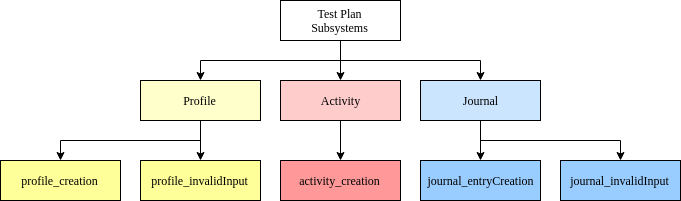
\includegraphics[scale=0.5]{../imgs/Figure2.png}
\caption{Overview of test plan subsystems and their associated test cases. (made using draw.io)}
\label{Figure2}
\end{figure}
\subsubsection{Profile}
The testing of this subsystem and the respective colorpicker.py, agepicker.py, and genderpicker.py files will begin with the creation of a test\textunderscore profile.py program with specific test\textunderscore profile\textunderscore creation and test\textunderscore profile\textunderscore invalidInput functions as test cases. These test cases go as follows:
\begin{enumerate}
\itemsep-0.5em
\item \textbf{test\textunderscore profile\textunderscore creation}: This function will consist of the selection of a valid color and a gender and the input of a valid age. The test will be passed if profile creation is carried through with according input and without the throwing of an exception.
\item \textbf{test\textunderscore profile\textunderscore invalidInput}: This function will consist of the input of an invalid color, gender, or age. The test will be passed if profile creation with this input throws an exception.
\end{enumerate}
\subsubsection{Journal}
The testing of this subsystem and the respective journalactivity.py, journalentry-bundle.py, and journalwindow.py files will begin with the creation of a test\textunderscore journal.py program with specific test\textunderscore journal\textunderscore entryCreation and test\textunderscore journal\textunderscore invalidInput functions as test cases. These test cases go as follows:
\begin{enumerate}
\itemsep-0.5em
\item \textbf{test\textunderscore journal\textunderscore entryCreation}: This function will consist of the opening of the journal entry window followed by the inputting of a valid journal entry name. The test will be passed if profile creation is carried through with according input and without the throwing of an exception.
\item \textbf{test\textunderscore journal\textunderscore invalidInput}: This function will consist of the opening of the journal entry window followed by the inputting of an invalid journal entry name (special characters, escaped characters, etc.). The test will be passed if profile creation with this input throws an exception.
\end{enumerate}
\subsubsection{Activity}
The testing of this subsystem and the respective buddy.py file will begin with the creation of a test\textunderscore activity.py program with specific test\textunderscore activity\textunderscore creation function as a test case. These test case goes as follows:
\begin{enumerate}
\itemsep-0.5em
\item \textbf{test\textunderscore activity\textunderscore creation}: This function will consist of the opening of the creation of a new activity and its assignment to a specific user profile. The test will be passed if activity creation is carried through with according input, assigned to the relevant profile, and without the throwing of an exception.
\end{enumerate}
\subsection{Testing Schedule}
The tentative schedule for our testing plan has been defined as follows:
\begin{itemize}
\itemsep-0.5em
\item[] \textbf{11/9/2018}: Completion of automated testing framework
\item[] \textbf{11/19/2018}: Completion of design and implementation of testing framework; Evaluation of twenty-five test cases
\item[] \textbf{11/28/2018}: Completion of code injection of 5 faults; Testing of chosen twenty-five test cases with faulty code.
\end{itemize}
\subsection{Test Recording Procedures}
Each of the implemented test cases will be coded in python and run through the terminal as described in the first deliverable. For easy auditing and understanding of previous tests, this code will include the date, time, and current software version with all output automatically being written to a log file for that specific date. These will be aggregated in a \textbf{testing} folder in the root directory of this testing framework's project.
\subsection{Hardware and Software Requirements}
As of the time of this document being written, Sugar Labs requires the local operating system to be either Debian 0.110 or higher, Fedora, or Ubuntu 16.04 or higher. In addition, Python 2.7, the main codebase of the software, must be installed alongside the sugar-artwork, sugar-datastore, and sugar-toolkit-gtk3 packages which can all be obtained directly from the terminal. For building the project, the packages intltool, libglib2.0-dev, and gtk+-3.0 should also be installed on the system. 
\subsection{Constraints}
Though there are not many constraints limiting the testing process of this project, we must plan to be punctual in every step of our testing framework's implementation as required by the general outline of this course. Due to the nature of this project (in it being carried out in an educational setting), we need not worry about budgeting, staff, or weekly meeting presentations, all of which are often necessitated in government or industry settings.
\subsection{System Tests}
The system tests will primarily consist of checking relevant software installations. The following software, shown with their according verification commands, will be used to check that the system is up-to-date and able to run SugarLabs:
\begin{itemize}
\itemsep-0.5em
\item \textbf{Python}: python -v
\item \textbf{intltool}: intltool -\--help
\item \textbf{autoconf}: autconf -h
\item \textbf{libglib2.0-dev}: dpkg -\--get-selections $\mid$ grep libglib2.0-dev
\item \textbf{gtk+-3.0}: dpkg -\--get-selections $\mid$ gtk-3.0
\end{itemize}
\subsection{Team Evaluation}
So far, our team seems to be making good progress. We’ve been able to properly install and make the source code that we pulled off of GitHub. We split our first test cases into three subsystems: Profile, Journal and Activity. We plan to put our future tests into each of these subsystems to make testing easier and more streamlined.Our goal is to test files required for profile creation, such as picking an age and gender, as well as assigning journal activities. 

\section{Deliverable 3: Automated Testing Framework}
\subsection{Architectural Description}
The automated testing framework has been subdivided in to following sections for ease of use:
\begin{itemize}[noitemsep,topsep=0pt]
\item[]\rotatebox[origin=c]{180}{$\Lsh$}\textbf{/TestAutomation}: Root directory for the automated testing framework
\begin{itemize}[noitemsep,topsep=0pt]
\item[]\rotatebox[origin=c]{180}{$\Lsh$}\textbf{/sugar}: Contains the cloned project files for the SugarLabs repository
\item[]\rotatebox[origin=c]{180}{$\Lsh$}\textbf{/scripts}: Contains scripts used for running a specific test case and for running all test cases
\item[]\rotatebox[origin=c]{180}{$\Lsh$}\textbf{/testCases}: Contains test case input
\item[]\rotatebox[origin=c]{180}{$\Lsh$}\textbf{/testCaseExecutables}: Contains the test cases written in python
\item[]\rotatebox[origin=c]{180}{$\Lsh$}\textbf{/temp}: Contains the output.log file where all testing output is piped
\item[]\rotatebox[origin=c]{180}{$\Lsh$}\textbf{/docs}: Contains the README.txt file for the automated testing framework
\item[]\rotatebox[origin=c]{180}{$\Lsh$}\textbf{/reports}: Contains all of the reports associated with the automated testing framework
\end{itemize}
\end{itemize}
\subsection{Documentation}
Each of the test cases have been written and saved to the /TestAutomation/testCaseExecutables folder, with their input files being located in /TestAutomation/testCases as described above. In each of these testCase input files is outlined a brief description of the test case and how one may go about modifying it for their own purposes. An example of such is provided in Figure \ref{Figure3}.
\begin{figure}
\centering
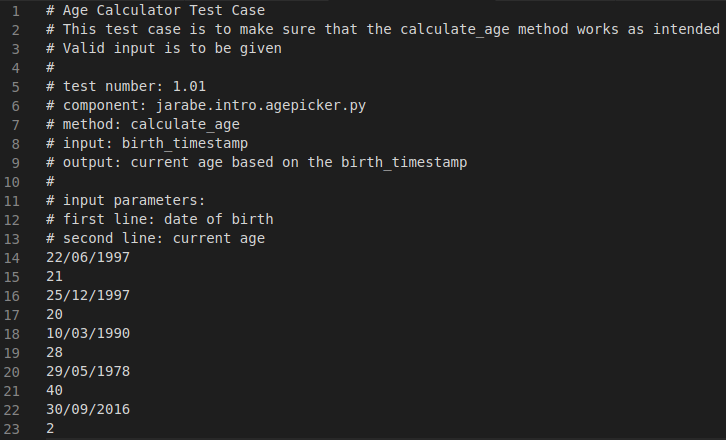
\includegraphics[scale=0.4]{../imgs/Figure3.png}
\caption{Example documentation for testCase input files, allowing users to be able to understand how to modify them as necessary.}
\label{Figure3}
\end{figure}
\subsection{Test Case Sepcifications}
For the first step in the implementation of our automate testing framework we wrote and exectuted five primary test cases. These are specified below.
\begin{enumerate}[noitemsep]
\item age\_calculator
\begin{itemize}[noitemsep,topsep=0pt]
\item \textbf{Test ID}: 2
\item \textbf{Test Requirement}: Correlated age input is properly recognized by the system as correct input and subsequently processed.
\item \textbf{Test Component}: jarabe.intro.agepicker
\item \textbf{Test Method}: calculate\_age
\item \textbf{Test Input}: Input is provided in the form of two-line input, the first being the birthdate of the user and the second the correct age of said user. Input: (22/06/1997, 21), (25/12/1997, 20), (10/03/1990, 28), (29/05/1978, 40), (30/09/2016, 2)
\item \textbf{Expected Output}: Output is expected to return True for each of the input test cases, as the calculated age and input age will match. Expected Output: True, True, True, True, True
\end{itemize}
\item age\_calculator\_invalid
\begin{itemize}[noitemsep,topsep=0pt]
\item \textbf{Test ID}: 3
\item \textbf{Test Requirement}: Noncorrelated age input is properly recognized by the system as incorrect input.
\item \textbf{Test Component}: jarabe.intro.agepicker
\item \textbf{Test Method}: calculate\_age
\item \textbf{Test Input}: Input is provided in the form of two-line input, the first being the birthdate of the user and the second the correct age of said user. Input: (22/06/1997, 22), (25/12/1997, 21), (10/03/1990, 29), (29/05/1978, 41), (30/09/2016, 3)
\item \textbf{Expected Output}: Output is expected to return False for each of the input test cases, as the calculated age and input age will match. Expected Output: False, False, False, False, False
\end{itemize}
\item buddy\_color
\begin{itemize}[noitemsep,topsep=0pt]
\item \textbf{Test ID}: 4
\item \textbf{Test Requirement}: A user must be able to set and be returned the color of their account's "buddy"
\item \textbf{Test Component}: jarabe.model.buddy
\item \textbf{Test Method}: set\_color, get\_color
\item \textbf{Test Input}: Input is provided in the form of a six-digit hex number, representing the buddy color. Input: FF00FF
\item \textbf{Expected Output}: Output is expected to return the input number for each of the input test cases, as the set method should properly set the color, and the get method should properly return the color. Expected Output: FF00FF
\end{itemize}
\item buddy\_key
\begin{itemize}[noitemsep,topsep=0pt]
\item \textbf{Test ID}: 5
\item \textbf{Test Requirement}: A user must be able to set and be returned the key of their account's "buddy"
\item \textbf{Test Component}: jarabe.model.buddy
\item \textbf{Test Method}: set\_key, get\_key
\item \textbf{Test Input}: Input is provided in the form of a two eight-letter codes joined by an underscore, representing the buddy key. Input: DEADBEEF\_DEADCODE
\item \textbf{Expected Output}: Output is expected to return the input key for each of the input test cases, as the set method should properly set the key, and the get method should properly return the key. Expected Output: DEADBEEF\_DEADCODE
\end{itemize}
\item buddy\_nickname
\begin{itemize}[noitemsep,topsep=0pt]
\item \textbf{Test ID}: 6
\item \textbf{Test Requirement}: A user must be able to set and be returned the nickname of their account's "buddy"
\item \textbf{Test Component}: jarabe.model.buddy
\item \textbf{Test Method}: set\_nick, get\_nick
\item \textbf{Test Input}: Input is provided in the form of a string, representing the buddy nickname. Input: bigboidan
\item \textbf{Expected Output}: Output is expected to return the input string for each of the input test cases, as the set method should properly set the nickname, and the get method should properly return the nickname. Expected Output: bigboidan
\end{itemize}
\end{enumerate}
\subsection{Team Evaluation}
This deliverable was definitely the most challenging task so far for this project. We decided to use python as out scripting language since that is what the project was written in to begin with, making it much easier to interact with the project files the sugarlabs team created. After creating a few test cases, we had some other issues to resolve like redirecting the output from unittests to a file instead of the terminal. Overall we are happy with the framework layout and our ability to create the rest of the test cases moving forward. 

\section{Deliverable 4: Complete Testing Specifications}
\subsection{Documentation}
As described in the previous section, the test cases have been implemented and saved into the directory structure as follows: each test case executable file has been saved in the /testing-framework/testCaseExecutables/ folder; each test case description has been saved in the /testing-framework/testCases/ folder; a short description as well as the inputs for the respective executable file have been documented in each of these text files.
\subsection{Test Case Specifications}
Below are detailed the specifications for all twenty-six test cases. Each brief description contains four main parts - the test case id number, the requirement being tested, the component being tested, and the method being testing.
\begin{enumerate}[noitemsep,topsep=0pt]
\item \textbf{Activity Chooser}:
\begin{itemize}[noitemsep,topsep=0pt]
\item \textbf{Test ID}: 1
\item \textbf{Requirement}: Checks ActivityChooser titles and constructor
\item \textbf{Component}: jarabe.model.activitychooser.py
\item \textbf{Method}: set\_title
\end{itemize}
\item \textbf{Age Calculator}:
\begin{itemize}[noitemsep,topsep=0pt]
\item \textbf{Test ID}: 2
\item \textbf{Requirement}: Checks for valid timestamp calculation of a birthdate
\item \textbf{Component}: jarabe.intro.agepicker.py
\item \textbf{Method}: calculate\_age
\end{itemize}
\item \textbf{Age Calculator Invalid}:
\begin{itemize}[noitemsep,topsep=0pt]
\item \textbf{Test ID}: 3
\item \textbf{Requirement}: Checks for invalid timestamp calculation of a birthdate
\item \textbf{Component}: jarabe.intro.agepicker.py
\item \textbf{Method}: calculate\_age
\end{itemize}
\item \textbf{Buddy Color}:
\begin{itemize}[noitemsep,topsep=0pt]
\item \textbf{Test ID}: 4
\item \textbf{Requirement}: Checks for color change ability
\item \textbf{Component}: jarabe.model.buddy.py
\item \textbf{Method}: set\_color
\end{itemize}
\item \textbf{Buddy Key}:
\begin{itemize}[noitemsep,topsep=0pt]
\item \textbf{Test ID}: 5
\item \textbf{Requirement}: Checks for key change ability
\item \textbf{Component}: jarabe.model.buddy.py
\item \textbf{Method}: set\_key
\end{itemize}
\item \textbf{Buddy Nickname}:
\begin{itemize}[noitemsep,topsep=0pt]
\item \textbf{Test ID}: 6
\item \textbf{Requirement}: Checks for nickname changes
\item \textbf{Component}: jarabe.model.buddy.py
\item \textbf{Method}: set\_nick
\end{itemize}
\item \textbf{Change Brightness}:
\begin{itemize}[noitemsep,topsep=0pt]
\item \textbf{Test ID}: 7
\item \textbf{Requirement}: Can set brightness levels
\item \textbf{Component}: jarabe.model.brightness.py
\item \textbf{Method}: set\_brightness
\end{itemize}
\item \textbf{CMD Help}:
\begin{itemize}[noitemsep,topsep=0pt]
\item \textbf{Test ID}: 8
\item \textbf{Requirement}: Testing system command line 
\item \textbf{Component}: jarabe.controlpanel.cmd.py
\item \textbf{Method}: cmd\_help
\end{itemize}
\item \textbf{CMD Restart}:
\begin{itemize}[noitemsep,topsep=0pt]
\item \textbf{Test ID}: 9
\item \textbf{Requirement}: Testing the system command line
\item \textbf{Component}: jarabe.controlpanel.cmd.py
\item \textbf{Method}: node\_restart
\end{itemize}
\item \textbf{Help Website}:
\begin{itemize}[noitemsep,topsep=0pt]
\item \textbf{Test ID}: 10
\item \textbf{Requirement}: Checks for the link to the help website
\item \textbf{Component}: jarabe.view.viewhelp.py
\item \textbf{Method}: get\_social\_help\_server
\end{itemize}
\item \textbf{HTTP Open}:
\begin{itemize}[noitemsep,topsep=0pt]
\item \textbf{Test ID}: 11
\item \textbf{Requirement}: Checks that http requests can be made
\item \textbf{Component}: jarabe.util.httprange.py
\item \textbf{Method}: open
\end{itemize}
\item \textbf{HTTP Size}:
\begin{itemize}[noitemsep,topsep=0pt]
\item \textbf{Test ID}: 12
\item \textbf{Requirement}: Checks that http requests are valid
\item \textbf{Component}: jarabe.util.httprange.py
\item \textbf{Method}: size
\end{itemize}
\item \textbf{Journal Comment}:
\begin{itemize}[noitemsep,topsep=0pt]
\item \textbf{Test ID}: 13
\item \textbf{Requirement}: Checks for journal comments
\item \textbf{Component}: jarabe.journal.expandedentry.py
\item \textbf{Method}: add\_row
\end{itemize}
\item \textbf{String isASCII}:
\begin{itemize}[noitemsep,topsep=0pt]
\item \textbf{Test ID}: 14
\item \textbf{Requirement}: Checks to make sure strings can be represented in ascii code
\item \textbf{Component}: jarabe.desktop.keydialog.py
\item \textbf{Method}: string\_is\_ascii
\end{itemize}
\item \textbf{String isHex}:
\begin{itemize}[noitemsep,topsep=0pt]
\item \textbf{Test ID}: 15
\item \textbf{Requirement}: Checks to make sure the hex string comparison is working
\item \textbf{Component}: jarabe.desktop.keydialog.py
\item \textbf{Method}: string\_is\_hex
\end{itemize}
\item \textbf{String Hex Converter}:
\begin{itemize}[noitemsep,topsep=0pt]
\item \textbf{Test ID}: 16
\item \textbf{Requirement}: Checks the string hex converter
\item \textbf{Component}: jarabe.desktop.keydialog.py
\item \textbf{Method}: string\_to\_hex
\end{itemize}
\item \textbf{Friends Model}:
\begin{itemize}[noitemsep,topsep=0pt]
\item \textbf{Test ID}: 17
\item \textbf{Requirement}: Checks for the friends model creation
\item \textbf{Component}: jarabe.model.friends.py
\item \textbf{Method}: get\_model
\end{itemize}
\item \textbf{Add Friend}:
\begin{itemize}[noitemsep,topsep=0pt]
\item \textbf{Test ID}: 18
\item \textbf{Requirement}: Checks for errors when adding a friend
\item \textbf{Component}: jarabe.model.friends.py
\item \textbf{Method}: add\_friend
\end{itemize}
\item \textbf{Has Friend}:
\begin{itemize}[noitemsep,topsep=0pt]
\item \textbf{Test ID}: 19
\item \textbf{Requirement}: Checks for added friends to appear as added
\item \textbf{Component}: jarabe.model.friends.py
\item \textbf{Method}: add\_friend
\end{itemize}
\item \textbf{String Normalization}:
\begin{itemize}[noitemsep,topsep=0pt]
\item \textbf{Test ID}: 20
\item \textbf{Requirement}: Tests string normalization (removing non-ascii characters)
\item \textbf{Component}: jarabe.util.normalize
\item \textbf{Method}: normalize
\end{itemize}
\item \textbf{Serial Number Generation}:
\begin{itemize}[noitemsep,topsep=0pt]
\item \textbf{Test ID}: 21
\item \textbf{Requirement}: Checks for randomized serial generation
\item \textbf{Component}: jarabe.model.session
\item \textbf{Method}: have\_systemd
\end{itemize}
\item \textbf{System Session Support}:
\begin{itemize}[noitemsep,topsep=0pt]
\item \textbf{Test ID}: 22
\item \textbf{Requirement}: Checks for school session logging support
\item \textbf{Component}: jarabe.model.session
\item \textbf{Method}: have\_systemd
\end{itemize}
\item \textbf{Get System Session}:
\begin{itemize}[noitemsep,topsep=0pt]
\item \textbf{Test ID}: 23
\item \textbf{Requirement}: Checks session logging
\item \textbf{Component}: jarabe.model.session
\item \textbf{Method}: get\_session
\end{itemize}
\item \textbf{Set Volume}:
\begin{itemize}[noitemsep,topsep=0pt]
\item \textbf{Test ID}: 24
\item \textbf{Requirement}: Changes the system volume
\item \textbf{Component}: jarabe.model.sound.py
\item \textbf{Method}: set\_volume
\end{itemize}
\item \textbf{Mute Volume}:
\begin{itemize}[topsep=0pt]
\item \textbf{Test ID}: 25
\item \textbf{Requirement}: Mutes the system volume
\item \textbf{Component}: jarabe.model.sound.py
\item \textbf{Method}: set\_muted
\end{itemize}
\item \textbf{Speech Manager}:
\begin{itemize}[noitemsep,topsep=0pt]
\item \textbf{Test ID}: 26
\item \textbf{Requirement}: Creates a speech manager utility
\item \textbf{Component}: jarabe.model.speed.py
\item \textbf{Method}: get\_speech\_manager
\end{itemize}
\end{enumerate}
\subsection{Team Evaluation}
In this deliverable our team had to finish flushing out all 25 of the test cases that our Testing Framework would be automatically testing as well as make any changes to the framework that we found necessary. We decided that the way the framework was set up was perfectly fine for the rest of the project. From here we had a large task ahead of us, planning out and executing 20 more test cases on top of the 5 that we had for the previous deliverable. We got off to a decent start knocking a few out pretty quickly and started to hit a bit of a wall. Our biggest problem was many of the classes and files this system used are graphical and required additional imports that were not needed for a successful build. That issue combined with the system being written in python, it made it very difficult to understand some of the files because even if we could get them imported for test cases, we were not sure what all of the parameters meant because of python being a dynamically typed language. We still managed to get all 25 test cases and some of them were able to test graphical components of the system without actually needing the graphics to appear on screen. Sugar Labs would is a great tool and idea, but with the lack of documentation and instructions it turned out to be much larger of a task to come in and get test cases written than we initially expected. Overall we are happy with what we have accomplished up to this point with the system, it would have just been much easier to understand Sugar Labs as a whole if the development team had more documentation throughout the code.

\section{Deliverable 5: Testing Fault-Injected Code}
\subsection{Description}
For this deliverable we have changed the code in multiple places inside of Sugar Labs’ system in order to make our testing framework fail on a few test cases. The changes could be removing method implementation, making mathematical mistakes and other changes to cause assertions to no longer be valid. This will help us further test out the framework to make sure that even with broken code, it does not cause our framework to crash
\subsection{Documentation}
When you first clone the directory, The full sugar labs source code will be in the ‘testing-framework/sugar’ directory, the working sugar labs files that we have not changed will be in the ‘testing-framework/scripts/fix/’ directory, and the faulty files will be in the ‘testing-framework/scripts/break/’ directory. 

To inject the faulty code, you will run the script ‘breakSugar.py’ from within the scripts directory. After breaking the code, you will need to run the ‘fixSugar.py’ script to get the original code back in the working sugar labs directory. Because of the sugar labs installation process, the code that is executed is actually found in the path: ‘/usr/local/lib/python2.7/dist-packages/jarabe/’.

When you run the fix or break scripts, we will be compiling the broken or fixed code, and replacing the files within this distribution folder. It is also possible that you will need to be root when you run the fix and break scripts.
\subsection{Changed Code}
The Sugar Labs software has been edited, as described in the preceding paragraphs, in the following source files with changes as described:
\begin{itemize}[noitemsep,topsep=0pt]
\item \textbf{agepicker.py}: Changed the \_SECONDS\_PER\_YEAR constant to $(365 * 24 * 60 * 60 * 60)$ instead of $(365 * 24 * 60 * 60)$ so our age calculation will no longer return the correct value, causing the age\_calculator test case.
\item \textbf{viewhelp.py}: Changed the ‘social-help-server’ string to ‘social-help’ in the get\_social\_help\_server method, so our help window will no longer be able to find the correct help web page, making the Help Website test case fail.
\item \textbf{httprange.py} Removed the line ‘self.\_size = self.\_result’ from the size method. This will make the size of the web request always return 0, so the users would never be able to tell if the http requests are even working. This will also cause our HTTP Size test case to fail for the method size.
\item \textbf{friends.py}: In the ‘has\_buddy’ method for a Friends object, we changed the check for ‘buddy.get\_key() in self.\_friends’ to not in friends. This makes the system think that people who are not friends are friends and vice versa. This will cause the has\_buddy method fail within our Buddy Check test case.
\item \textbf{schoolserver.py}: In the \_generate\_serial\_number() we added a line to seed the random number generator so that this serial number creator is no longer random. In our test case we have the seed match what the system usually used, so now our Serial Number test case will fail
\end{itemize}
\subsection{Team Evaluation}
For this deliverable we have changed the code in multiple places inside of Sugar Labs’ system in order to make our testing framework fail on a few test cases. The changes could be removing method implementation, making mathematical mistakes and other changes to cause assertions to no longer be valid. This will help us further test out the framework to make sure that even with broken code, it does not cause our framework to crash. This wasn't too difficult to plan out, the hardest part was replacing the actual sugar labs code. After installation Sugar Labs installs everything to the python distributable folder on your computer with the compiled files. To accompany these installations, we wrote scripts files to compile our changed code and replace the files in the sugar install directory. We also wrote a script file to replace the original code.

\section{Overall Experiences}

\end{document}